\documentclass[12pt]{article}

%***************************************************************************************************
% Math
\usepackage{fancyhdr} 
\usepackage{amsfonts}
\usepackage{amsmath}
\usepackage{amssymb}
\usepackage{amsthm}
%\usepackage{dsfont}

%***************************************************************************************************
% Macros
\usepackage{calc}

%***************************************************************************************************
% Commands and Custom Variables	
\newcommand{\problem}[1]{\hspace{-4 ex} \large \textbf{Problem #1} }
\let\oldemptyset\emptyset
\let\emptyset\varnothing
\newcommand{\norm}[1]{\left\lVert#1\right\rVert}
\newcommand{\sint}{\text{s}\kern-5pt\int}
\newcommand{\powerset}{\mathcal{P}}
\renewenvironment{proof}{\hspace{-4 ex} \emph{Proof}:}{\qed}
\newcommand{\RR}{\mathbb{R}}
\newcommand{\NN}{\mathbb{N}}
\newcommand{\QQ}{\mathbb{Q}}
\newcommand{\ZZ}{\mathbb{Z}}
\newcommand{\CC}{\mathbb{C}}

\let\vec\mathbf


%***************************************************************************************************
%page
\usepackage[margin=1in]{geometry}
\usepackage{setspace}
%\doublespacing
\allowdisplaybreaks
\pagestyle{fancy}
\fancyhf{}
\rhead{Shaw \space \thepage}
%\setlength\parindent{0pt}

%***************************************************************************************************
%Code
\usepackage{listings}
\usepackage{courier}
\lstset{
	language=Python,
	showstringspaces=false,
	formfeed=newpage,
	tabsize=4,
	commentstyle=\itshape,
	basicstyle=\ttfamily,
}

%***************************************************************************************************
%Images
\usepackage{graphicx}
\graphicspath{ {images/} }
\usepackage{float}


\title{Pre-Proposal\\ \large Solving PDEs using Radial Basis Function Finite Difference Methods in Parallel}
\author{Student: Sage Shaw\\ Advisor: Prof. Grady Wright}
\date{April 2, 2018}

%\renewcommand{\abstractname}{Overview}

\usepackage[backend=bibtex, style=numeric, sorting=none]{biblatex}
\addbibresource{pre-proposal.bib}
%\bibliography{SRF}


\begin{document}
	\thispagestyle{empty}
	
	\begin{flushright}
		Sage Shaw \\
		m566 - Spring 2018 \\
		\today
	\end{flushright}
	
	%{\large \textbf{Pre-Proposal}}\bigbreak
	\begin{center}
		\Huge \textbf{Pre-Proposal} \\
		\large Solving PDEs using RBF-FD in Parallel
	\end{center}

\section{Problem Statement} 
Finite difference methods are numerical techniques for finding solutions to PDEs that approximate the solution on a mesh of points that are equally spaced across the domain. In situations where the desired points are not on a mesh, or when the domain does not lend itself to simple meshes, it is desirable to have mesh-free methods. Radial Basis Function Finite Differnence methods (RBF-FD) are such mesh-free methods. 

For this project we intend to explore parallelization of RBF-FD methods. We begin with a summary of standard finite differences applied to steady-state PDEs. We then compare with the basic RBF-FD method. 

\subsection{Review of the standard Finite Difference Method} 
The standard finite difference approach to solving PDEs relies on using a grid of points over the domain that have an equal spacing $h$ (the step size) in each direction. Taylor's theorem is used to generate finite difference formulae that approximate the derivative at a point in terms of the surrounding points. For example, consider the one dimensional steady state heat equation, $\frac{d^2u}{dx^2} = g(x)$. The second order finite difference approximation is given by

$$
\frac{d^2u}{dx^2}(x_i) \approx \frac{1}{h^2}u(x_{i-1}) - \frac{2}{h^2} u(x_i) + \frac{1}{h^2} u(x_{i+1}),
$$
where $x_i$ denotes the $i$th equally spaced point on the domain.

Using finite difference approximation at every point on the grid the problem is reduced to a system of equations (often sparse) involving $g(x)$ and any boundary conditions. In the case of our example we get the system $C\vec{u} = \vec{f}$ where $\vec{u}$ is an approximation of $u(x)$ at grid points, $\vec{f}$ is a vector containing information from the forcing term $g(x)$ and the boundary conditions, and $C$ is given by
\begin{align*}
	C = 
	\frac{1}{h^2}\begin{bmatrix}
		-2 & 1  &     &   &  &  &\\
		1 & -2 &  1  &   &  &  &\\
		& 1  &  -2 & 1 &  &  &\\
		&    & \ddots & \ddots & \ddots&\\
		&    &     & 1 & -2 & 1  \\
		&    &     &   &  1 & -2
	\end{bmatrix}
\end{align*}
We can rewrite our PDE more generally as $L(u(x))=g(x)$ where $L$ is a linear differential operator. Here the matrix $C$ is a discrete approximation of $L$ in the same sense that $\vec{u}$ is an approximation of $u(x)$ at the grid points.

\subsection{Overview of RBF-FD}	
As discussed in Fornberg \& Flyer (2015)\cite{Fornberg2015} the RBF-FD method generalizes this idea. We forgo the mesh in favor of an arbitrary set of distinct points $\{x_i\}_{i=1}^n$. We then would like to form the linear system $C\vec{u} = \vec{g}$ so that $C$ approximates $L$ at each point in our set. Here $C$ is not derived from a finite difference formula, but instead computed. We choose a set of basis functions $\{\phi_j\}_{j=1}^n$ and ensure that for every point $x_i$
\begin{align}
	L(\phi_j)(x_i) = \sum\limits_{j=1}^{n} c_{i,j} \phi_j(x_i) \phantom{===} \text{for } j=1,...,n \label{row_coef}
\end{align}
In other words we require that our weighted sum of $\{\phi_j\}_{j=1}^n$ approximates $L$ acting on each of our basis functions at each point in our set. Once $C$ is formed, we have reduced the problem to that of solving the linear system $C\vec{u} = \vec{g}$. \bigbreak

%The Marihuber-Curtis theorem \cite{Mairhuber1956}\cite{Curtis1959} proves that the matrix $C$ may, in general, be singular. However, if $\{\phi_j\}_{j=1}^n$ are chosen to be radial basis functions centered at our points then we are guaranteed that the system is non-singular. \bigbreak

As a demonstration consider the boundary value partial differential equation
\begin{align}
	\frac{d^2u}{dx^2} &= \frac{-9\pi^2}{5}\sin(3\pi x), & u(0)&=2, & u(1)&=3 \label{PDE1D}
\end{align}
Figure \ref{1Dsolutions} shows the true solution to (\ref{PDE1D}) in blue along with the RBF-FD solutions using $n=5,10,25, \text{and } 50$ points in the interior. Even with very few points the approximation is quite close. \bigbreak

A significant advantage of RBF-FD methods is that the formulation does not depend on the domain. Nearly the exact same algorithm can be applied to 2-dimensional problems. \bigbreak

\begin{figure}[ht]
	\caption{1 dimensional RBF-FD solutions to (\ref{PDE1D})}
	\begin{tabular}{cc}
		\includegraphics[width=.4\textwidth]{1D_n5} & \includegraphics[width=.4\textwidth]{1D_n10} \\
		n=5 & n=10 \\
		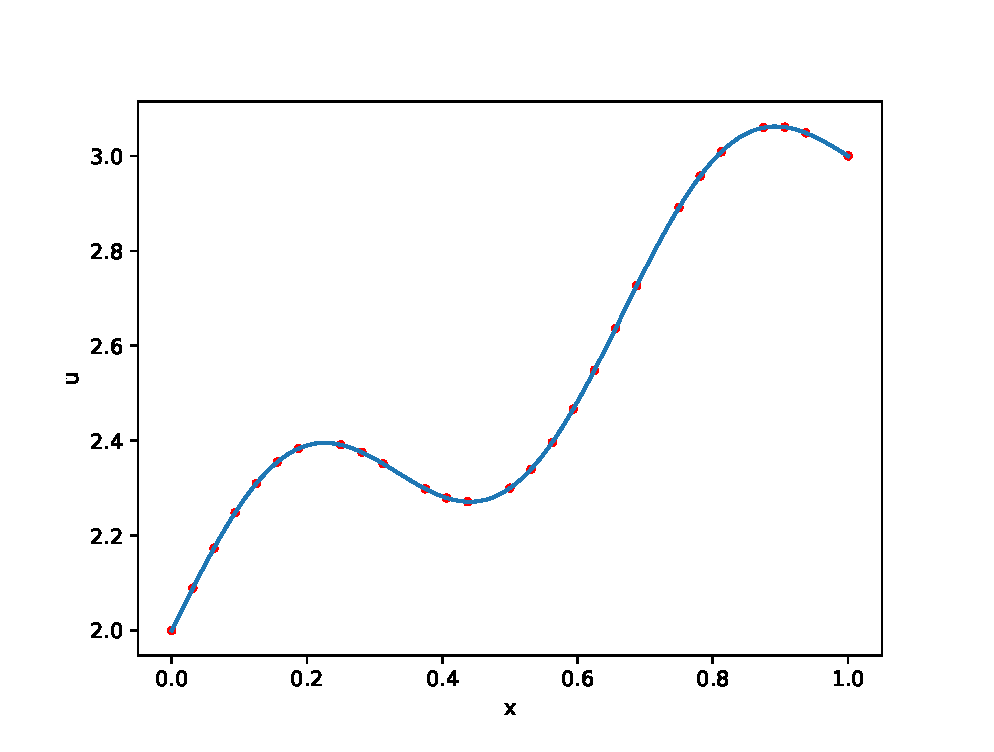
\includegraphics[width=.4\textwidth]{1D_n25} & 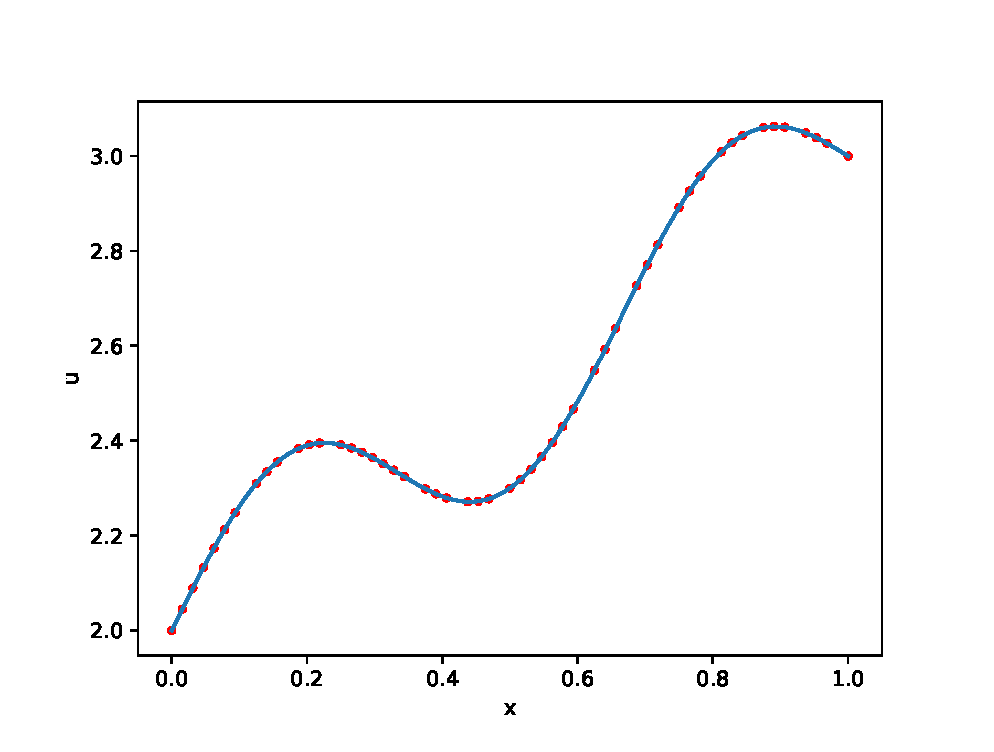
\includegraphics[width=.4\textwidth]{1D_n50} \\
		n=25 & n=50
	\end{tabular}
	\label{1Dsolutions}
	\centering
\end{figure}

For example, consider the 2-dimensional boundary value problem (Poisson's equation) on the unit disk
\begin{align}
	\frac{\partial ^2u}{\partial x^2} + \frac{\partial ^2u}{\partial y^2} &= 0, & u(x,y)&=(y-0.1)^2 \text{ on the boundary}  \label{PDE2D}
\end{align}
The RBF-FD solution can be seen in figure \ref{2Dsolutions} for $n$ points in the interior and sampled at $b$ points on the boundary.

At a given point, it is reasonable to assume that the weights used to approximate the derivative for far off points should be small - essentially that local function values are weighted heavier in the approximation of the derivative. This motivates the idea to use only local points for the calculations of the weights in equation (\ref{row_coef}). In this case we used the $l$-nearest neighbors for each point meaning that each row of $C$ has only $l$ non-zero entries. For large numbers of points, this can dramatically reduce the computational cost of calculating the weights, and also ensures that $C$ is sparse. 

\begin{figure}[ht]
	\caption{Solution to (\ref{PDE2D}) using $n$ interior points (black), $b$ boundary points (gold), and a stencil size of $l$ nearest neighbors}
	\begin{tabular}{cc}
		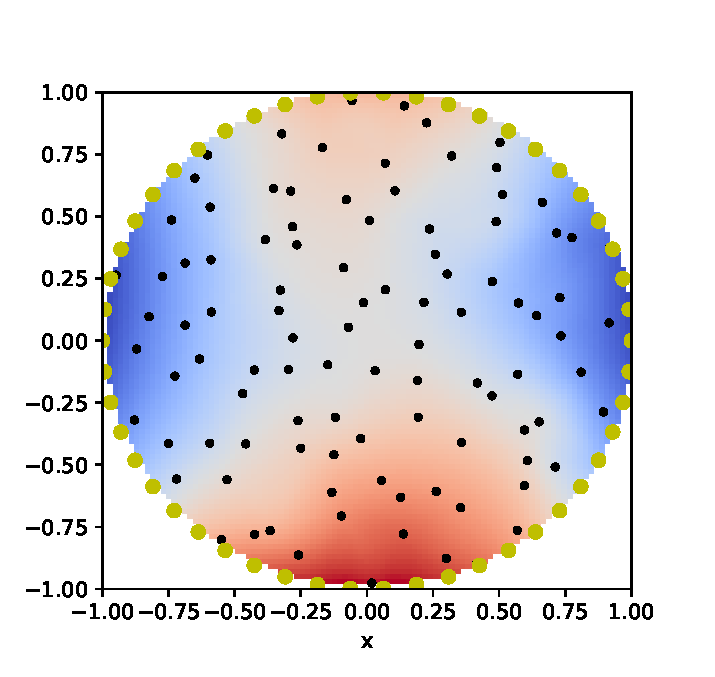
\includegraphics[width=.5\textwidth]{2D_n100_b50} & 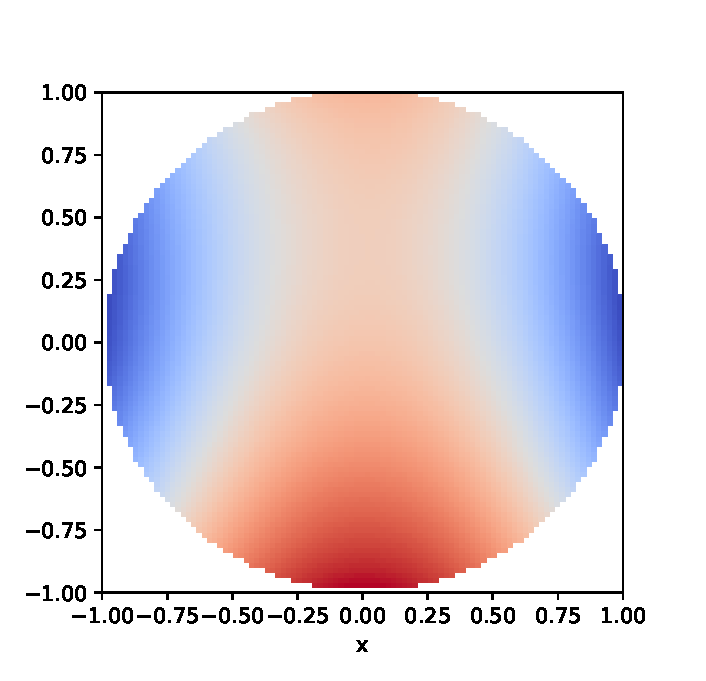
\includegraphics[width=.5\textwidth]{2D_n2000_b50_l50} \\
		n=100 \phantom{==} b=50 \phantom{==} l=5 & n=2000 \phantom{==} b=50 \phantom{==} l=50 
	\end{tabular}
	\label{2Dsolutions}
	\centering
\end{figure}

%%%%%%%%%%%%%%%%%%%%%%%%%%%%%%%%%%%%%%%%%%%%%%%%%%%%%%%%%%%%%%%%%%%%%%%%%%%%%
%%%%%%%%%%%%%%%%%%%%%%%%%%%%%%%%%%%%%%%%%%%%%%%%%%%%%%%%%%%%%%%%%%%%%%%%%%%%%
%%%%%%%%%%%%%%%%%%%%%%%%%%%%%%%%%%%%%%%%%%%%%%%%%%%%%%%%%%%%%%%%%%%%%%%%%%%%%

\section{Existing Solutions}
	The primary solution we will attempt to emulate is from Bollig, Flyer \& Erlebacher (2012)\cite{Bollig2012}. Here, they apply RBF-FD parallelized over muliple CPUs and GPUs. The domain of the problem is divided up among CPU-GPU pairs. The differentiation weights matrix is calculated once in serial and the weights for corresponding points, as well as the initial values at those points are then distributed to their CPU-GPU pairs. The CPUs handle synchronization and communication between processes and the GPUs are used to calculate the time-steps.
	
	Since 2012 there have been advancements in RBF-FD methods that were not available. In particular work has been done using particular RBFs that do not require a shape parameter but do require additional basis functions. This has been explored in 
	Flyer et al.(2016)\cite{Flyer2016-1}\cite{Flyer2017-2} and in Barnett \& Wicker (2016)\cite{FlyerBarnettWicker2016}, however they did not implement their techniques in parallel.
	
%%%%%%%%%%%%%%%%%%%%%%%%%%%%%%%%%%%%%%%%%%%%%%%%%%%%%%%%%%%%%%%%%%%%%%%%%%%%%
%%%%%%%%%%%%%%%%%%%%%%%%%%%%%%%%%%%%%%%%%%%%%%%%%%%%%%%%%%%%%%%%%%%%%%%%%%%%%
%%%%%%%%%%%%%%%%%%%%%%%%%%%%%%%%%%%%%%%%%%%%%%%%%%%%%%%%%%%%%%%%%%%%%%%%%%%%%


\section{Proposed Innovation}
	The solution in Bollig, Flyer \& Erlebacher (2012)\cite{Bollig2012} assumed that the domain and pointset were fixed and thus the differentiation matrix would be the same over each time-step making the cost of computing it negligible compared to the cost of performing the time steps. They decided to perform this calculation in serial. We would like to parallelize this step as well, to allow the algorithm to be adapted to problems with time-dependent domains.
	
	Their calculation of the differentiation matrix uses a technique that allows the approximation to exactly reproduce a constant. This method has been extended as in Flyer et al.\cite{Flyer2016-1}\cite{Flyer2017-2} to exactly reproduce polynomials up to a specified degree. This method also encourages the use of polyharmonic spline RBFs which don't require a shape parameter. We would like to incorporate these advancements.
 
% \bigbreak
\pagebreak
 
\printbibliography

\end{document}
